\chapter{Agenda y Turnos}
\label{mod:04-agenda-turnos}

\section{Propósito}
\label{sec:agenda-proposito}

Gestiona el calendario de turnos entre pacientes y profesionales: reserva por parte de recepción/staff, auto-reserva del propio paciente desde el portal (self-booking), disponibilidad del profesional (horarios semanales, pausas, bloqueos puntuales) y el ciclo de confirmación/cancelación de un turno. Es la puerta de entrada habitual a una \code{ConsultaClinica}.

\section{Entidades principales}
\label{sec:agenda-entidades}

\begin{longtable}{p{3.2cm}p{11.5cm}}
\caption{Entidades principales del módulo de Agenda.}
\label{tab:agenda-entidades}\\
\toprule
\textbf{Entidad} & \textbf{Rol} \\
\midrule
\endfirsthead
\toprule
\textbf{Entidad} & \textbf{Rol} \\
\midrule
\endhead
\bottomrule
\endfoot
\code{Turno} & El turno en sí: paciente, profesional, sucursal, fecha/hora, estado. Ver Capítulo~\ref{sec:modelo-datos} (Grupo B). \\
\code{Horario}\allowbreak \code{Profesional} & Disponibilidad semanal recurrente de un profesional, por sucursal. Ver Capítulo~\ref{sec:modelo-datos} (Grupo A). \\
\code{PausaHorario} & Ventana de pausa dentro de un \code{Horario}\allowbreak \code{Profesional} (ej.\ almuerzo). Ver Capítulo~\ref{sec:modelo-datos} (Grupo A). \\
\code{BloqueoFecha} & Excepción puntual a la disponibilidad (ej.\ vacaciones, feriado). Ver Capítulo~\ref{sec:modelo-datos} (Grupo A). \\
\code{EstadoConfig} & Estado cosmético configurable (color/nombre) para \code{Turno.}\allowbreak \code{EstadoCustomId}, no gobierna la lógica. Ver Capítulo~\ref{sec:modelo-datos} (Grupo B). \\
\end{longtable}

\section{Reglas de negocio clave}
\label{sec:agenda-reglas}

\begin{itemize}
  \item \textbf{\code{Turno.Estado} (enum \code{TurnoEstado}) es la fuente de verdad de la lógica}; \code{EstadoCustomId} (FK a \code{EstadoConfig}) es puramente cosmético/configurable por el negocio (color, nombre visible) y no la reemplaza.
  \item \textbf{Un paciente solo puede tener un turno activo a la vez.} ``Activo'' = \code{Pendiente}, \code{Confirmado} o \code{Presente}. Un turno \code{Completado} no cuenta como activo (corrección explícita: antes bloqueaba con cualquier estado no cancelado, incluido \code{Completado}, dejando al paciente sin poder reservar nunca más tras su primera consulta).
  \item \textbf{Self-booking exige \code{SucursalId} obligatorio} en \code{Self}\allowbreak \code{Book}\allowbreak \code{Turno}\allowbreak \code{Request} --- impacto directo del proyecto multi-sucursal, ver \hyperref[adr:0009]{ADR 0009 --- Sucursal fija por usuario}. El paciente, al ser global (sin sucursal propia), elige la sucursal en el momento de reservar.
  \item \textbf{\code{Horario}\allowbreak \code{Profesional} está scopeado por sucursal}, con índice único \code{ProfessionalId + SucursalId + DiaSemana} --- un mismo profesional puede tener horarios distintos en cada sucursal donde atiende.
  \item \textbf{Policy \code{ver_disponibles} es un OR} (\code{ver_agenda} del staff \textbf{o} \code{ver_mis_turnos} del paciente) --- permite que ambos perfiles consulten slots libres sin exponerle al paciente el resto de la agenda.
  \item \textbf{Confirmación por token de email:} \code{POST /api/turnos/confirmar/{token}} es público (\code{AllowAnonymous}) --- el paciente confirma el turno desde el link del email sin necesidad de estar logueado.
  \item \textbf{Cancelación en dos pasos:} el paciente solo puede \emph{solicitar} la cancelación (\code{solicitar-cancelacion}, marca \code{Turno.SolicitudCancelacion = true}); el staff es quien la resuelve (\code{gestionar-cancelacion}, aprueba o rechaza). El paciente nunca cancela directamente su propio turno.
  \item \textbf{Recordatorios automáticos:} \code{Turno}\allowbreak \code{Reminder}\allowbreak \code{Service} (\code{BackgroundService}, ver Capítulo~\ref{sec:arch}, \S\ref{sec:arch-background-services}) envía recordatorios por email antes del turno.
\end{itemize}

\section{Endpoints}
\label{sec:agenda-endpoints}

\begin{longtable}{p{2cm}p{6.4cm}p{6.4cm}}
\caption{Endpoints principales del módulo de Agenda.}
\label{tab:agenda-endpoints}\\
\toprule
\textbf{Método} & \textbf{Ruta} & \textbf{Descripción} \\
\midrule
\endfirsthead
\toprule
\textbf{Método} & \textbf{Ruta} & \textbf{Descripción} \\
\midrule
\endhead
\bottomrule
\endfoot
GET & \code{/api/turnos} & Listado filtrado (staff) \\
GET & \code{/}\allowbreak \code{api/}\allowbreak \code{turnos/}\allowbreak \code{disponibles} & Slots libres (staff u paciente, policy OR) \\
GET & \code{/}\allowbreak \code{api/}\allowbreak \code{turnos/}\allowbreak \code{profesionales-disponibles} & Profesionales con horario activo ese día (paso 1 del self-booking) \\
POST & \code{/api/turnos} & Alta manual (staff) \\
PUT & \code{/api/turnos/{id}/estado} & Cambio de estado \\
GET/POST & \code{/}\allowbreak \code{api/}\allowbreak \code{turnos/}\allowbreak \code{mis-turnos}, \code{/}\allowbreak \code{api/}\allowbreak \code{turnos/}\allowbreak \code{self-book} & Portal del paciente \\
POST & \code{/api/turnos/{id}/}\allowbreak \code{solicitar-cancelacion}, \code{/}\allowbreak \code{gestionar-cancelacion} & Cancelación en dos pasos \\
POST & \code{/}\allowbreak \code{api/}\allowbreak \code{turnos/}\allowbreak \code{confirmar/}\allowbreak \code{{token}} & Confirmación pública por email \\
GET/PUT & \code{/}\allowbreak \code{api/}\allowbreak \code{professionals/}\allowbreak \code{{id}/horarios}, \code{/bloqueos} & Disponibilidad del profesional (\code{Horarios}\allowbreak \code{Controller}) \\
\end{longtable}

Detalle completo (policies, DTOs) en el Apéndice de Referencia de API, \S~4 Agenda.

\section{Flujo típico}
\label{sec:agenda-flujo}

Self-booking desde el portal del paciente, dividido en dos figuras por cantidad de pasos.

\begin{figure}[htbp]
\centering
\begin{tikzpicture}
  \node[actor] (p) at (0,0) {Paciente\\\footnotesize MisTurnosView};
  \node[actor] (api) at (4,0) {TurnosController};
  \node[actor] (svc) at (8.4,0) {TurnoService};
  \node[actor] (db) at (12.2,0) {PostgreSQL};

  \draw[lineavida] (p.south) -- ++(0,-7.2);
  \draw[lineavida] (api.south) -- ++(0,-7.2);
  \draw[lineavida] (svc.south) -- ++(0,-7.2);
  \draw[lineavida] (db.south) -- ++(0,-7.2);

  \draw[mensaje] ($(p.south)+(0,-0.8)$) -- node[above,font=\scriptsize]{GET /turnos/profesionales-disponibles} ($(api.south)+(0,-0.8)$);
  \draw[mensaje] ($(api.south)+(0,-1.6)$) -- node[above,font=\scriptsize]{GetProfesionalesDisponiblesAsync} ($(svc.south)+(0,-1.6)$);
  \draw[mensaje] ($(svc.south)+(0,-2.4)$) -- node[above,font=\scriptsize]{horario activo ese día} ($(db.south)+(0,-2.4)$);
  \draw[mensajeretorno] ($(api.south)+(0,-3.2)$) -- node[above,font=\scriptsize]{lista de profesionales} ($(p.south)+(0,-3.2)$);

  \draw[mensaje] ($(p.south)+(0,-4.2)$) -- node[above,font=\scriptsize]{GET /turnos/disponibles?...} ($(api.south)+(0,-4.2)$);
  \draw[mensajeretorno] ($(api.south)+(0,-5.0)$) -- node[above,font=\scriptsize]{slots libres} ($(p.south)+(0,-5.0)$);

  \draw[mensaje] ($(p.south)+(0,-6.0)$) -- node[above,font=\scriptsize]{POST /turnos/self-book (SucursalId oblig.)} ($(api.south)+(0,-6.0)$);
  \draw[mensaje] ($(api.south)+(0,-6.8)$) -- node[above,font=\scriptsize]{SelfBookAsync} ($(svc.south)+(0,-6.8)$);
\end{tikzpicture}
\caption{Self-booking: búsqueda de disponibilidad y reserva (parte 1 de 2).}
\label{fig:seq-agenda-selfbook-1}
\end{figure}

\begin{figure}[htbp]
\centering
\begin{tikzpicture}
  \node[actor] (p) at (0,0) {Paciente};
  \node[actor] (api) at (4,0) {TurnosController};
  \node[actor] (svc) at (8.4,0) {TurnoService};
  \node[actor] (db) at (12.2,0) {PostgreSQL};

  \draw[lineavida] (p.south) -- ++(0,-5.6);
  \draw[lineavida] (api.south) -- ++(0,-5.6);
  \draw[lineavida] (svc.south) -- ++(0,-5.6);
  \draw[lineavida] (db.south) -- ++(0,-5.6);

  \draw[mensaje] ($(svc.south)+(0,-0.8)$) -- node[above,font=\scriptsize]{valida sin turno activo} ($(db.south)+(0,-0.8)$);
  \draw[mensaje] ($(svc.south)+(0,-1.6)$) -- node[above,font=\scriptsize]{crea Turno (Estado=Pendiente)} ($(db.south)+(0,-1.6)$);
  \draw[mensajeretorno] ($(svc.south)+(0,-2.4)$) -- node[above,font=\scriptsize]{email con link de confirmación} ($(p.south)+(0,-2.4)$);

  \draw[mensaje] ($(p.south)+(0,-3.6)$) -- node[above,font=\scriptsize]{POST /turnos/confirmar/{token} (AllowAnonymous)} ($(api.south)+(0,-3.6)$);
  \draw[mensaje] ($(api.south)+(0,-4.4)$) -- node[above,font=\scriptsize]{Turno.Estado = Confirmado} ($(db.south)+(0,-4.4)$);
\end{tikzpicture}
\caption{Self-booking: creación del turno y confirmación por email (parte 2 de 2).}
\label{fig:seq-agenda-selfbook-2}
\end{figure}

Cancelación: el paciente solicita (\code{solicitar-cancelacion}) $\rightarrow$ el staff ve la bandera \code{Solicitud}\allowbreak \code{Cancelacion} en \code{AgendaView} $\rightarrow$ aprueba o rechaza (\code{gestionar-cancelacion}).

\section{Vistas de frontend}
\label{sec:agenda-vistas}

\begin{itemize}
  \item \code{AgendaView.vue} --- agenda del staff.
  \item \code{MisTurnosView.vue} --- portal del paciente: calendario mensual propio (grilla 7$\times$6, sin librería externa), modal de reserva en dos pasos (profesional $\to$ horario), respeta la regla de ``un solo turno activo''.
  \item \code{ConfirmarTurnoView.}\allowbreak \code{vue} --- landing pública del link de confirmación por email.
  \item La gestión de horarios/pausas/bloqueos del profesional no tiene vista propia --- vive embebida en \code{ProfesionalesView.}\allowbreak \code{vue}.
\end{itemize}

\section{Interfaz}
\label{sec:agenda-interfaz}

\begin{figure}[htbp]
\centering
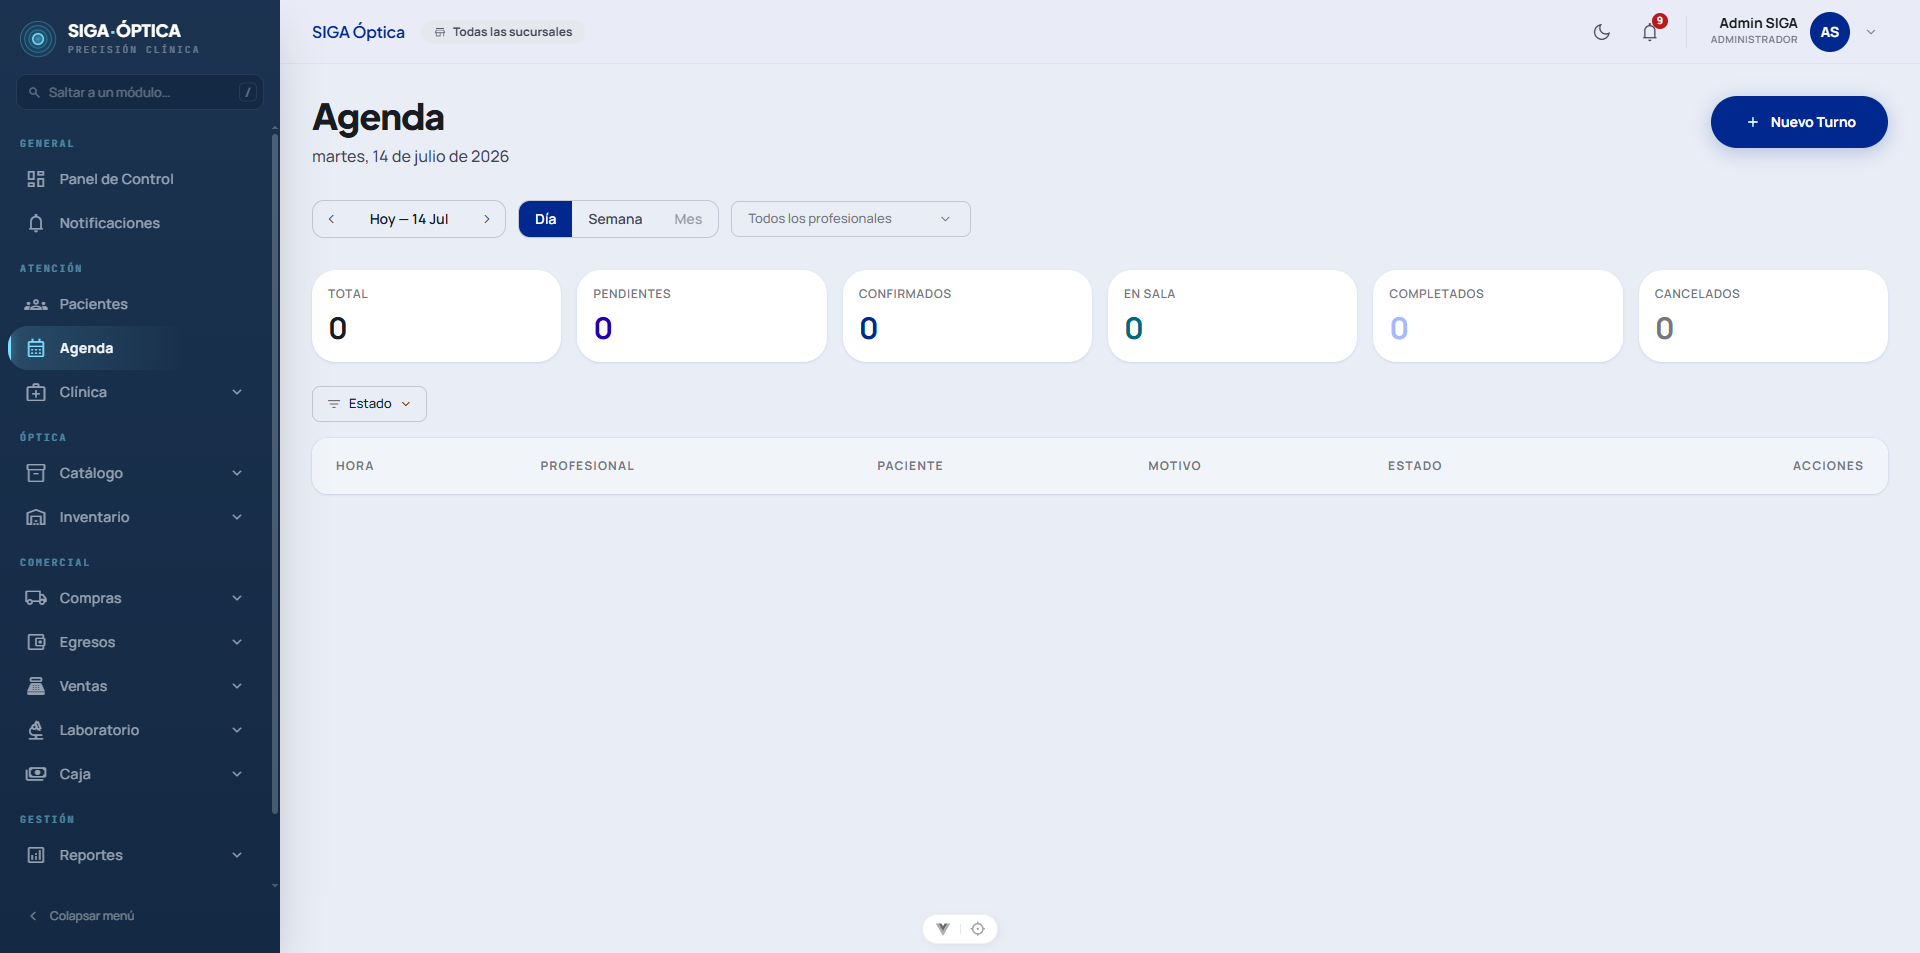
\includegraphics[width=0.95\textwidth]{imagenes/mod04-agenda.png}
\caption{Agenda de turnos del día, con los contadores de estado (pendientes, confirmados, en sala, completados, cancelados) y el filtro por profesional.}
\label{fig:mod04-agenda}
\end{figure}

\section{Estado}
\label{sec:agenda-estado}

\Implementado, incluyendo self-booking, confirmación por email y scoping multi-sucursal (Fase 4 del proyecto de sucursales).
